% Intended LaTeX compiler: pdflatex


\documentclass[12pt]{article}
% \usepackage[includeheadfoot,margin=1.0in,hmargin=1.0in,vmargin=0.5in]{geometry} % for normal margins
\usepackage[includeheadfoot,margin=1.5in,hmargin=1.5in,vmargin=0.5in]{geometry} % for insanely wide margins
% \usepackage[includeheadfoot,margin=2.0in,hmargin=2.0in,vmargin=0.5in]{geometry} % for insanely wide margins
\usepackage{float}


\usepackage{algorithm}
\usepackage{amsmath}
\usepackage{ifxetex}
\ifxetex
  \usepackage{fontspec,xltxtra,xunicode}
  \defaultfontfeatures{Mapping=tex-text,Scale=MatchLowercase}
  \setromanfont{Garamond Premier Pro}
%  \setromanfont{Adobe Caslon Pro}
 \setsansfont{Gotham Narrow Bold}
  \setmonofont{Myriad Pro}
\else
  \usepackage[mathletters]{ucs}
  \usepackage[utf8x]{inputenc}
\fi
\usepackage{url}
\usepackage{paralist}
\usepackage{graphicx}
\usepackage{tikz}
\usepackage{calc}
\usepackage{eso-pic}
\usepackage{etoolbox}
\usepackage{xcolor}
\PassOptionsToPackage{hyperref,x11names}{xcolor}
\definecolor{pinterestred}{HTML}{C92228}
\definecolor{ulyssesbutterflyblue}{HTML}{1464F4}
\definecolor{signalflare}{HTML}{FB782C}
\definecolor{niceorange}{HTML}{77CC6D}
\definecolor{highlighteryellow}{HTML}{FFFF01}
\definecolor{ghostlygrey}{HTML}{000000}
\definecolor{firstcolor}{HTML}{00ADEF}
\definecolor{secondcolor}{HTML}{DD3E74}
\definecolor{periodblue}{HTML}{12239e}
\definecolor{denimblue}{HTML}{3A5F90}
\definecolor{electricblue}{HTML}{05ADF3}


\newtoks\leftheader 
\newtoks\leftheaderurl
\newtoks\coverimage


\hyphenpenalty=5000 
\tolerance=1000

%This macro is to make cleaner the specification of the titling font
\newfontfamily\mytitlefont[Color={highlighteryellow}]{Gotham Narrow Bold}
\newfontfamily\myauthorfont[Color={highlighteryellow}]{Gotham Narrow Bold}
\newfontfamily\mybluefont[Color=electricblue]{Gotham Narrow Bold}
\DeclareTextFontCommand{\textbf}{\bfseries\color{electricblue}}
\DeclareTextFontCommand{\textit}{\itshape}


\usepackage{textcase}

\pagenumbering{arabic}
\makeatletter

%This macro now controls the position of the background pic
%Please do not change from here
\newcommand\BackgroundPic{%
\put(0,0){%
\parbox[b][\paperheight]{\paperwidth}{%
\vfill
\centering
%inside the tikzpicture environment, you can do anything you want with the image
\begin{tikzpicture}

\node [inner sep=0pt,outer sep=0pt] at (0,0) {\includegraphics[width=\paperwidth,height=\paperheight]{\the\coverimage}};

\node at  (0,5) [opacity=1.0] {\parbox[b][0.5\textheight]{\textwidth}{%
  \begin{raggedright}
  \leavevmode
    \vskip 1cm
  {\mytitlefont\fontsize{75}{85}\bfseries{\@title}\par}
    \vskip 1cm
    
    %{\myauthorfont\fontsize{30}{40}{{\bfseries{\@degree}\par}}}

\vfill
\end{raggedright}}};
\node at (0,-8) [opacity=1] {\parbox[b][0.3\textheight]{\textwidth}{%
\begin{raggedright}
\vfill
{\myauthorfont\Large {\@author}}
    \newline
          {\myauthorfont\Large \href{mailto:jay@storytelling.nyc}{jay@storytelling.nyc}}
        \newline
{\myauthorfont\Large
\href{http://storytelling.nyc}{Storytelling.NYC}}
\newline
{\myauthorfont\Large © 2017 \@author}
    \newline
%{\myauthorfont\Large Private and Confidential}
 %   \newline
        \newline
    {\myauthorfont\Large \@date\par}
%{\myauthorfont\Large \href{http://jaydixit.com}{\@degree }}
\end{raggedright}
}};
\end{tikzpicture}
%Don't change
\vfill
}}}
%This macro executes a hook at the beginning of the document that  puts the background correctly. 
\AtBeginDocument{\AddToShipoutPicture*{\BackgroundPic}}
\AtBeginDocument{\globalcolor{ghostlygrey}}



%The maketitle macro now only includes the titling and not the background. 
\def\maketitle{ \newgeometry{margin=1in} \thispagestyle{empty} \vfill \null \cleardoublepage\restoregeometry}



\setcounter{secnumdepth}{0}




\usepackage{fancyhdr}
\pagestyle{fancy}
\renewcommand{\sectionmark}[1]{\markboth{#1}{}}
\lhead{\href{\the\leftheaderurl}{\the\leftheader}}
\chead{}
\rhead{\@title: {\nouppercase{\leftmark}}}
\lfoot{}
\cfoot{}
\rfoot{}
\usepackage{listings}
\setlength{\parindent}{0pt}
\setlength{\parskip}{12pt plus 2pt minus 1pt} %Space between paragraphs
\usepackage{fancyvrb}
\usepackage{enumerate}
\usepackage{ctable}
\setlength{\paperwidth}{8.5in}
\setlength{\paperheight}{11in}
  \tolerance=1000
\usepackage{tocloft}
\renewcommand{\cftsecleader}{\cftdotfill{\cftdotsep}}
\usepackage[normalem]{ulem}


\makeatletter
\newcommand{\globalcolor}[1]{%
  \color{#1}\global\let\default@color\current@color
}
\makeatother

\newcommand{\textsubscr}[1]{\ensuremath{_{\scriptsize\textrm{#1}}}}

\usepackage{enumitem}
\newlist{mylist}{enumerate}{10} 
%\setlist{nolistsep}
\setlist{topsep=0pt}
\renewcommand{\labelitemi}{\raise 0.25ex\hbox{\tiny$\bullet$}}
\renewcommand{\labelitemii}{\raise 0.25ex\hbox{\tiny$\bullet$}}
\renewcommand{\labelitemiii}{\raise 0.25ex\hbox{\tiny$\bullet$}}
\renewcommand{\labelitemiv}{\raise 0.25ex\hbox{\tiny$\bullet$}}
\renewcommand{\labelitemv}{\raise 0.25ex\hbox{\tiny$\bullet$}}
\renewcommand{\labelitemvi}{\raise 0.25ex\hbox{\tiny$\bullet$}}
\renewcommand{\labelitemvii}{\raise 0.25ex\hbox{\tiny$\bullet$}}
\renewcommand{\labelitemviii}{\raise 0.25ex\hbox{\tiny$\bullet$}}
\renewcommand{\labelitemix}{\raise 0.25ex\hbox{\tiny$\bullet$}}
\renewcommand{\labelitemx}{\raise 0.25ex\hbox{\tiny$\bullet$}}

\setlistdepth{10}
\setlist[itemize,1]{label=\raise 0.25ex\hbox\tiny$\bullet$}
\setlist[itemize,2]{label=\raise 0.25ex\hbox\tiny$\bullet$}
\setlist[itemize,3]{label=\raise 0.25ex\hbox\tiny$\bullet$}
\setlist[itemize,4]{label=\raise 0.25ex\hbox\tiny$\bullet$}
\setlist[itemize,5]{label=\raise 0.25ex\hbox\tiny$\bullet$}
\setlist[itemize,6]{label=\raise 0.25ex\hbox\tiny$\bullet$}
\setlist[itemize,7]{label=\raise 0.25ex\hbox\tiny$\bullet$}
\setlist[itemize,8]{label=\raise 0.25ex\hbox\tiny$\bullet$}
\setlist[itemize,9]{label=\raise 0.25ex\hbox\tiny$\bullet$}
\setlist[itemize,10]{label=\raise 0.25ex\hbox\tiny$\bullet$}
\renewlist{itemize}{itemize}{10}





\definecolor{azure}{HTML}{f2feff}

\usepackage{lipsum}
\usepackage{tikz}
\usetikzlibrary{backgrounds}
\makeatletter

\tikzset{%
  fancy quotes/.style={
    text width=\fq@width pt,
    align=justify,
    inner sep=1em,
    anchor=north west,
    minimum width=\linewidth,
  },
  fancy quotes width/.initial={.8\linewidth},
  fancy quotes marks/.style={
    scale=8,
    text=black,
    inner sep=0pt,
  },
  fancy quotes opening/.style={
    fancy quotes marks,
  },
  fancy quotes closing/.style={
    fancy quotes marks,
  },
  fancy quotes background/.style={
    show background rectangle,
    inner frame xsep=0pt,
    background rectangle/.style={
      fill=azure,
      rounded corners,
    },
  }
}

\newenvironment{fancyquotes}[1][]{%
\noindent
\tikzpicture[fancy quotes background]
\node[fancy quotes opening,anchor=north west] (fq@ul) at (0,0) {``};
\tikz@scan@one@point\pgfutil@firstofone(fq@ul.east)
\pgfmathsetmacro{\fq@width}{\linewidth - 2*\pgf@x}
\node[fancy quotes,#1] (fq@txt) at (fq@ul.north west) \bgroup}
{\egroup;
\node[overlay,fancy quotes closing,anchor=east] at (fq@txt.south east) {''};
\endtikzpicture}
\makeatother


\usepackage{setspace}
\usepackage{lipsum}
\usepackage{etoolbox}
\AtBeginEnvironment{quote}{\singlespace\vspace{-\topsep}\small}
\AtEndEnvironment{quote}{\vspace{-\topsep}\endsinglespace}


\usepackage[sc]{titlesec}
\titlespacing*{\section}{0pt}{6pt}{7pt}
\titlespacing*{\subsection}{0pt}{0pt}{7pt}
\titlespacing*{\subsubsection}{0pt}{6pt}{5pt}

\titleformat*{\section}{\normalfont\fontsize{36}{36}\raggedright\bfseries\sffamily\color{pinterestred}}
\titleformat*{\subsection}{\normalfont\fontsize{20}{20}\scshape\color{electricblue}}
\titleformat*{\subsubsection}{\normalfont\fontsize{12}{8}\raggedright\bfseries\rmfamily\color{pinterestred}}
\titleformat*{\paragraph}{\normalfont\normalsize\raggedright\bfseries\rmfamily\color{electricblue}}
\titleformat*{\subparagraph}{\normalfont\fontsize{14}{14}\raggedright\bfseries\ttfamily\color{pinterestred}}
\usepackage[breaklinks=true,linktocpage,xetex]{hyperref} 
\hypersetup{colorlinks, citecolor=electricblue,filecolor=electricblue,linkcolor=electricblue,urlcolor=electricblue}




      

\setcounter{secnumdepth}{0}
\setcounter{tocdepth}{3}
\leftheader{Jay Dixit}
\leftheaderurl{http://jaydixit.com}
\coverimage{/Users/jay/emacs/emacs-settings/new-latex-templates/images/image1.jpg}
\author{Jay Dixit Jay Dixit}
\date{\today}
\title{Effective Emails Effective Emails}
\hypersetup{
 pdfauthor={Jay Dixit Jay Dixit},
 pdftitle={Effective Emails Effective Emails},
 pdfkeywords={},
 pdfsubject={},
 pdfcreator={Emacs 25.1.1 (Org mode 9.1.2)}, 
 pdflang={English}}
\begin{document}

\maketitle
\tableofcontents
\newpage


\section[Effective Emails]{Effective Emails\hfill{}\textsc{slide:aligncenter}}
\label{sec:org3a01c78}

\textbf{Jay Dixit} \\
\href{http://www.storytelling.nyc}{www.storytelling.nyc} \\
\href{mailto:jay@storytelling.nyc}{jay@storytelling.nyc} \\

\begin{center}

\includegraphics[width=.9\linewidth]{/Users/jay/Dropbox/github/org-html-webslides/assets/img/storytelling-nyc-logo-new-face.png}
\end{center}

\section[Agenda]{Agenda\hfill{}\textsc{slide:wrap:bgwhite:shadow:fancynumberedlist}}
\label{sec:orgd27d402}
\begin{enumerate}
\item Review of storytelling framework
\item Other structures for persuasive emails
\item Clarity and concision
\item Review of homework: Problem, Agitation, Solution
\end{enumerate}

\section[Jay's Elements of \textbf{Storytelling}]{Jay's Elements of \textbf{Storytelling}\hfill{}\textsc{slide:invisible:full}}
\label{sec:org72f6910}
\begin{center}
\includegraphics[width=.9\linewidth]{/Users/jay/Dropbox/storytelling-assets/images/presto-rabbit-cage-desire-goal-obstacle.jpg}
\end{center}


\section[Jay's Elements of \textbf{Storytelling}]{Jay's Elements of \textbf{Storytelling}\hfill{}\textsc{slide:wrap:bgwhite:shadow:fancynumberedlist:compressed:image10}}
\label{sec:org6065d26}

\begin{enumerate}
\item Goal \begin{center}

\includegraphics[width=.9\linewidth]{/Users/jay/Dropbox/github/org-html-webslides/assets/storytelling-icons/goal.png}
\end{center}
\item Obstacle \begin{center}

\includegraphics[width=.9\linewidth]{/Users/jay/Dropbox/github/org-html-webslides/assets/storytelling-icons/obstacle.png}
\end{center}
\end{enumerate}



\section[Stakes]{Stakes\hfill{}\textsc{slide:image30}}
\label{sec:org9b5b73a}

\begin{center}

\includegraphics[width=.9\linewidth]{/Users/jay/Dropbox/github/org-html-webslides/assets/storytelling-icons/stakes.png}
\end{center}

\section[Stakes]{Stakes\hfill{}\textsc{slide:full:invisible}}
\label{sec:org6c327de}

\begin{center}
\includegraphics[width=.9\linewidth]{/Users/jay/Dropbox/storytelling-assets/images/hangover-what-is-goal.jpg}
\end{center}


\section[Stakes]{Stakes\hfill{}\textsc{slide:full:invisible}}
\label{sec:org43b36e2}

\begin{center}
\includegraphics[width=.9\linewidth]{/Users/jay/Dropbox/storytelling-assets/images/hangover-phone-call-stakes.jpg}
\end{center}

\section[Stakes]{Stakes\hfill{}\textsc{slide:full:invisible}}
\label{sec:org81de412}

\begin{center}
\includegraphics[width=.9\linewidth]{/Users/jay/Dropbox/storytelling-assets/images/hangover-bride-angry.png}
\end{center}


\section[Stakes]{Stakes\hfill{}\textsc{slide:full:invisible}}
\label{sec:org7cfe57d}

\begin{center}
\includegraphics[width=.9\linewidth]{/Users/jay/Dropbox/storytelling-assets/images/hangover-bride-and-family.png}
\end{center}

\section[Jay's Elements of \textbf{Storytelling}]{Jay's Elements of \textbf{Storytelling}\hfill{}\textsc{slide:wrap:bgwhite:shadow:fancynumberedlist:compressed:image10}}
\label{sec:org9d3508b}

\begin{enumerate}
\item Goal \begin{center}

\includegraphics[width=.9\linewidth]{/Users/jay/Dropbox/github/org-html-webslides/assets/storytelling-icons/goal.png}
\end{center}
\item Obstacle \begin{center}

\includegraphics[width=.9\linewidth]{/Users/jay/Dropbox/github/org-html-webslides/assets/storytelling-icons/obstacle.png}
\end{center}
\item Stakes \begin{center}

\includegraphics[width=.9\linewidth]{/Users/jay/Dropbox/github/org-html-webslides/assets/storytelling-icons/stakes.png}
\end{center}
\end{enumerate}

\section[Strategies]{Strategies\hfill{}\textsc{slide:image30}}
\label{sec:org3271ca3}
\begin{center}

\includegraphics[width=.9\linewidth]{/Users/jay/Dropbox/github/org-html-webslides/assets/storytelling-icons/strategies.png}
\end{center}

\section[Strategies]{Strategies\hfill{}\textsc{slide:full:invisible:darkbloom}}
\label{sec:org572dc8f}

\begin{center}
\includegraphics[width=.9\linewidth]{/Users/jay/Dropbox/storytelling-assets/Bourne-Identity-006.jpg}
\end{center}

\section{Outcome                          :slide:image30: \begin{center}

\includegraphics[width=.9\linewidth]{/Users/jay/Dropbox/github/org-html-webslides/assets/storytelling-icons/outcome.png}
\end{center}}
\label{sec:org59be3d6}

\section[Outcome]{Outcome\hfill{}\textsc{slide:full:invisible}}
\label{sec:org2253bea}
\begin{center}
\includegraphics[width=.9\linewidth]{/Users/jay/Dropbox/storytelling-assets/images/success-outcome-victory-summit.jpg}
\end{center}

\section[The Storytelling.NYC Method]{The Storytelling.NYC Method\hfill{}\textsc{slide:wrap:bgwhite:shadow:fancynumberedlist:compressed:image10}}
\label{sec:org48b5b93}
\begin{enumerate}
\item Goal \begin{center}

\includegraphics[width=.9\linewidth]{/Users/jay/Dropbox/github/org-html-webslides/assets/storytelling-icons/goal.png}
\end{center}
\item Obstacle \begin{center}

\includegraphics[width=.9\linewidth]{/Users/jay/Dropbox/github/org-html-webslides/assets/storytelling-icons/obstacle.png}
\end{center}
\item Stakes \begin{center}

\includegraphics[width=.9\linewidth]{/Users/jay/Dropbox/github/org-html-webslides/assets/storytelling-icons/stakes.png}
\end{center}
\item Strategies \begin{center}

\includegraphics[width=.9\linewidth]{/Users/jay/Dropbox/github/org-html-webslides/assets/storytelling-icons/strategies.png}
\end{center}
\item Outcome \begin{center}

\includegraphics[width=.9\linewidth]{/Users/jay/Dropbox/github/org-html-webslides/assets/storytelling-icons/outcome.png}
\end{center}
\end{enumerate}

\section[The \textbf{shapes} of \textbf{stories}]{The \textbf{shapes} of \textbf{stories}\hfill{}\textsc{slide}}
\label{sec:org1c0f9ee}

\section[The \textbf{shapes} of \textbf{stories}]{The \textbf{shapes} of \textbf{stories}\hfill{}\textsc{slide}}
\label{sec:org6272b72}
\begin{center}
\includegraphics[width=.9\linewidth]{/Users/jay/Dropbox/storytelling-assets/charts/kurt-vonnegut--the-shapes-of-stories-all-the-kinds.jpeg}
\end{center}
\section[The \textbf{shapes} of \textbf{stories}]{The \textbf{shapes} of \textbf{stories}\hfill{}\textsc{slide}}
\label{sec:org35d3e70}
\begin{center}
\includegraphics[width=.9\linewidth]{/Users/jay/Dropbox/storytelling-assets/charts/kurt-vonnegut--the-shapes-of-stories-all-the-kinds-1.jpeg}
\end{center}

\section[Man falls in a hole]{Man falls in a hole\hfill{}\textsc{slide:image80}}
\label{sec:orge3338a7}
\begin{center}
\includegraphics[width=.9\linewidth]{/Users/jay/Dropbox/storytelling-assets/charts/details/man-in-hole.png}
\end{center}

\section[The Castaway]{The Castaway\hfill{}\textsc{slide:full:invisible}}
\label{sec:orgcd8c77c}
\url{http://i.ytimg.com/vi/MLnzF5NcAc4/maxresdefault.jpg}

\section[The Castaway]{The Castaway\hfill{}\textsc{slide:full:invisible}}
\label{sec:org1f5f170}
\url{https://i.ytimg.com/vi/ZbunWKwRg9o/maxresdefault.jpg}

\section[The Castaway]{The Castaway\hfill{}\textsc{slide:full:invisible}}
\label{sec:orgbdd21c7}
\url{http://ak5.picdn.net/shutterstock/videos/4000456/thumb/4.jpg}

\section[The Castaway]{The Castaway\hfill{}\textsc{slide:full:invisible}}
\label{sec:org0583d6f}
\url{http://i.huffpost.com/gen/2581364/images/o-TOM-HANKS-CAST-AWAY-facebook.jpg}

\section[The Castaway]{The Castaway\hfill{}\textsc{slide:full:invisible}}
\label{sec:org7e1b8db}
\url{https://i.ytimg.com/vi/7bLQXZOzjFM/maxresdefault.jpg}

\section[Man falls in a hole]{Man falls in a hole\hfill{}\textsc{slide:image80}}
\label{sec:org2497390}
\begin{center}
\includegraphics[width=.9\linewidth]{/Users/jay/Dropbox/storytelling-assets/charts/details/man-in-hole.png}
\end{center}

\section[A structure for a persuasive email]{A structure for a persuasive email\hfill{}\textsc{slide:wrap:bgwhite:shadow:fancynumberedlist:compressed:image30}}
\label{sec:org871ef79}
\begin{enumerate}
\item Problem \begin{center}

\includegraphics[width=.9\linewidth]{/Users/jay/Dropbox/github/org-html-webslides/assets/img/3d-problem.png}
\end{center}
\item Agitation \begin{center}
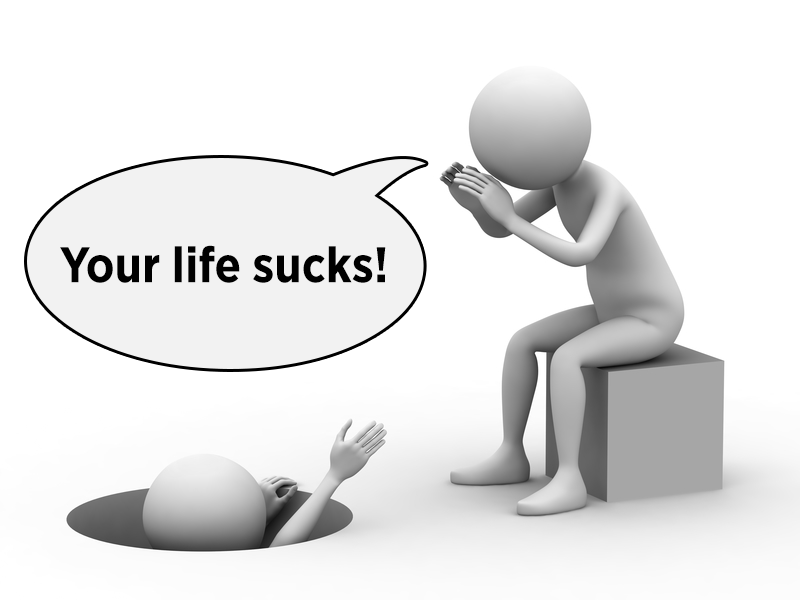
\includegraphics[width=.9\linewidth]{/Users/jay/Dropbox/github/org-html-webslides/assets/img/3d-agitation-your-life-sucks.png}
\end{center}
\item Solution \begin{center}
\includegraphics[width=.9\linewidth]{/Users/jay/Dropbox/storytelling-assets/images/3d-solution.jpg}
\end{center}
\end{enumerate}

\section[A structure for a persuasive email]{A structure for a persuasive email\hfill{}\textsc{slide}}
\label{sec:org67a9106}
\begin{center}
\begin{tabular}{ll}
\hline
Storytelling & Sales Email\\
\hline
Goal/Obstacle & Problem\\
Stakes & Agitation\\
Strategy & Solution\\
\hline
\end{tabular}
\end{center}

\section[The \textbf{shape} of a \textbf{story}]{The \textbf{shape} of a \textbf{story}\hfill{}\textsc{slide}}
\label{sec:orgf173fd7}
\section[The \textbf{shape} of a \textbf{story}]{The \textbf{shape} of a \textbf{story}\hfill{}\textsc{slide:image80}}
\label{sec:org18137f0}
\begin{center}
\includegraphics[width=.9\linewidth]{/Users/jay/Dropbox/storytelling-assets/charts/details/boy-meets-girl.png}
\end{center}

\section[Boy meets girl]{Boy meets girl\hfill{}\textsc{slide:image80}}
\label{sec:orgcdb5b84}
\begin{center}
\includegraphics[width=.9\linewidth]{/Users/jay/Dropbox/storytelling-assets/charts/details/boy-meets-girl.png}
\end{center}

\section[Boy meets girl]{Boy meets girl\hfill{}\textsc{slide:full:invisible}}
\label{sec:orga571b3a}
\url{https://metrouk2.files.wordpress.com/2016/07/ad\_214181254-e1469715492453.jpg}

\section[Boy meets girl]{Boy meets girl\hfill{}\textsc{slide:full:invisible}}
\label{sec:org72fd23e}
\url{https://typeset-beta.imgix.net/rehost\%2F2016\%2F9\%2F13\%2Fbd80ab25-9ca1-44be-9bd0-669a3066134e.png}

\section[Boy meets girl]{Boy meets girl\hfill{}\textsc{slide:full:invisible}}
\label{sec:org0cccc5f}
\url{http://lwlcdn.lwlies.com/wp-content/uploads/2016/01/romeo-and-juliet-1996.jpg}

\section[A structure for a persuasive email]{A structure for a persuasive email\hfill{}\textsc{slide:wrap:bgwhite:shadow:fancynumberedlist:compressed:image20}}
\label{sec:org9280e2e}
\begin{enumerate}
\item Opportunity \begin{center}
\includegraphics[width=.9\linewidth]{/Users/jay/Dropbox/storytelling-assets/images/icons/noun_diamond-object-of-desire.png}
\end{center}
\item Benefits \begin{center}
\includegraphics[width=.9\linewidth]{/Users/jay/Dropbox/storytelling-assets/images/icons/benefits-icon.png}
\end{center}
\item Solution \begin{center}
\includegraphics[width=.9\linewidth]{/Users/jay/Dropbox/storytelling-assets/images/icons/solution-icon.png}
\end{center}
\end{enumerate}

\section[1. Opportunity]{1. Opportunity\hfill{}\textsc{slide:image60}}
\label{sec:org74bc0e6}
\begin{center}
\includegraphics[width=.9\linewidth]{/Users/jay/Dropbox/storytelling-assets/images/icons/noun_diamond-object-of-desire.png}
\end{center}


\section[2. Benefits]{2. Benefits\hfill{}\textsc{slide:image60}}
\label{sec:org448d992}
\begin{center}
\includegraphics[width=.9\linewidth]{/Users/jay/Dropbox/storytelling-assets/images/icons/benefits-icon.png}
\end{center}


\section[3. Solution]{3. Solution\hfill{}\textsc{slide:image60}}
\label{sec:orgd69a793}
\begin{center}
\includegraphics[width=.9\linewidth]{/Users/jay/Dropbox/storytelling-assets/images/icons/solution-icon.png}
\end{center}


\section[A structure for a persuasive email]{A structure for a persuasive email\hfill{}\textsc{image20}}
\label{sec:org23458e4}
\begin{center}
\begin{tabular}{ll}
\hline
Storytelling & Sales Email\\
\hline
object of desire \begin{center}
\includegraphics[width=.9\linewidth]{/Users/jay/Dropbox/storytelling-assets/images/icons/woman-object-of-desire.png}
\end{center} & Opportunity                                                              \begin{center}
\includegraphics[width=.9\linewidth]{/Users/jay/Dropbox/storytelling-assets/images/icons/noun_diamond-object-of-desire.png}
\end{center}\\
Stakes                                                      \begin{center}

\includegraphics[width=.9\linewidth]{/Users/jay/Dropbox/github/org-html-webslides/assets/storytelling-icons/stakes.png}
\end{center} & Benefits                                                              \begin{center}
\includegraphics[width=.9\linewidth]{/Users/jay/Dropbox/storytelling-assets/images/icons/benefits-icon.png}
\end{center}\\
Strategy                                          \begin{center}

\includegraphics[width=.9\linewidth]{/Users/jay/Dropbox/github/org-html-webslides/assets/storytelling-icons/strategies.png}
\end{center} & Solution \begin{center}
\includegraphics[width=.9\linewidth]{/Users/jay/Dropbox/storytelling-assets/images/icons/solution-icon.png}
\end{center}\\
 & \\
 & \\
 & \\
\hline
\end{tabular}
\end{center}

\section[Exercise: Opportunity / Benefits / Solution]{Exercise: Opportunity / Benefits / Solution\hfill{}\textsc{slide:image80}}
\label{sec:orgbe52f34}
How can you apply the Opportunity / Benefits / Solution framework in your own outgoing emails?



\section[A structure for a persuasive email]{A structure for a persuasive email\hfill{}\textsc{slide}}
\label{sec:orgf203d4a}
\begin{center}
\begin{tabular}{ll}
\hline
Storytelling & Sales Email\\
\hline
Goal (object of desire) & Opportunity\\
Stakes & Benefits\\
Strategy & Solution\\
\hline
\end{tabular}
\end{center}

\section[Avoiding information \textbf{overload}]{Avoiding information \textbf{overload}\hfill{}\textsc{slide}}
\label{sec:org72279f2}
\begin{center}
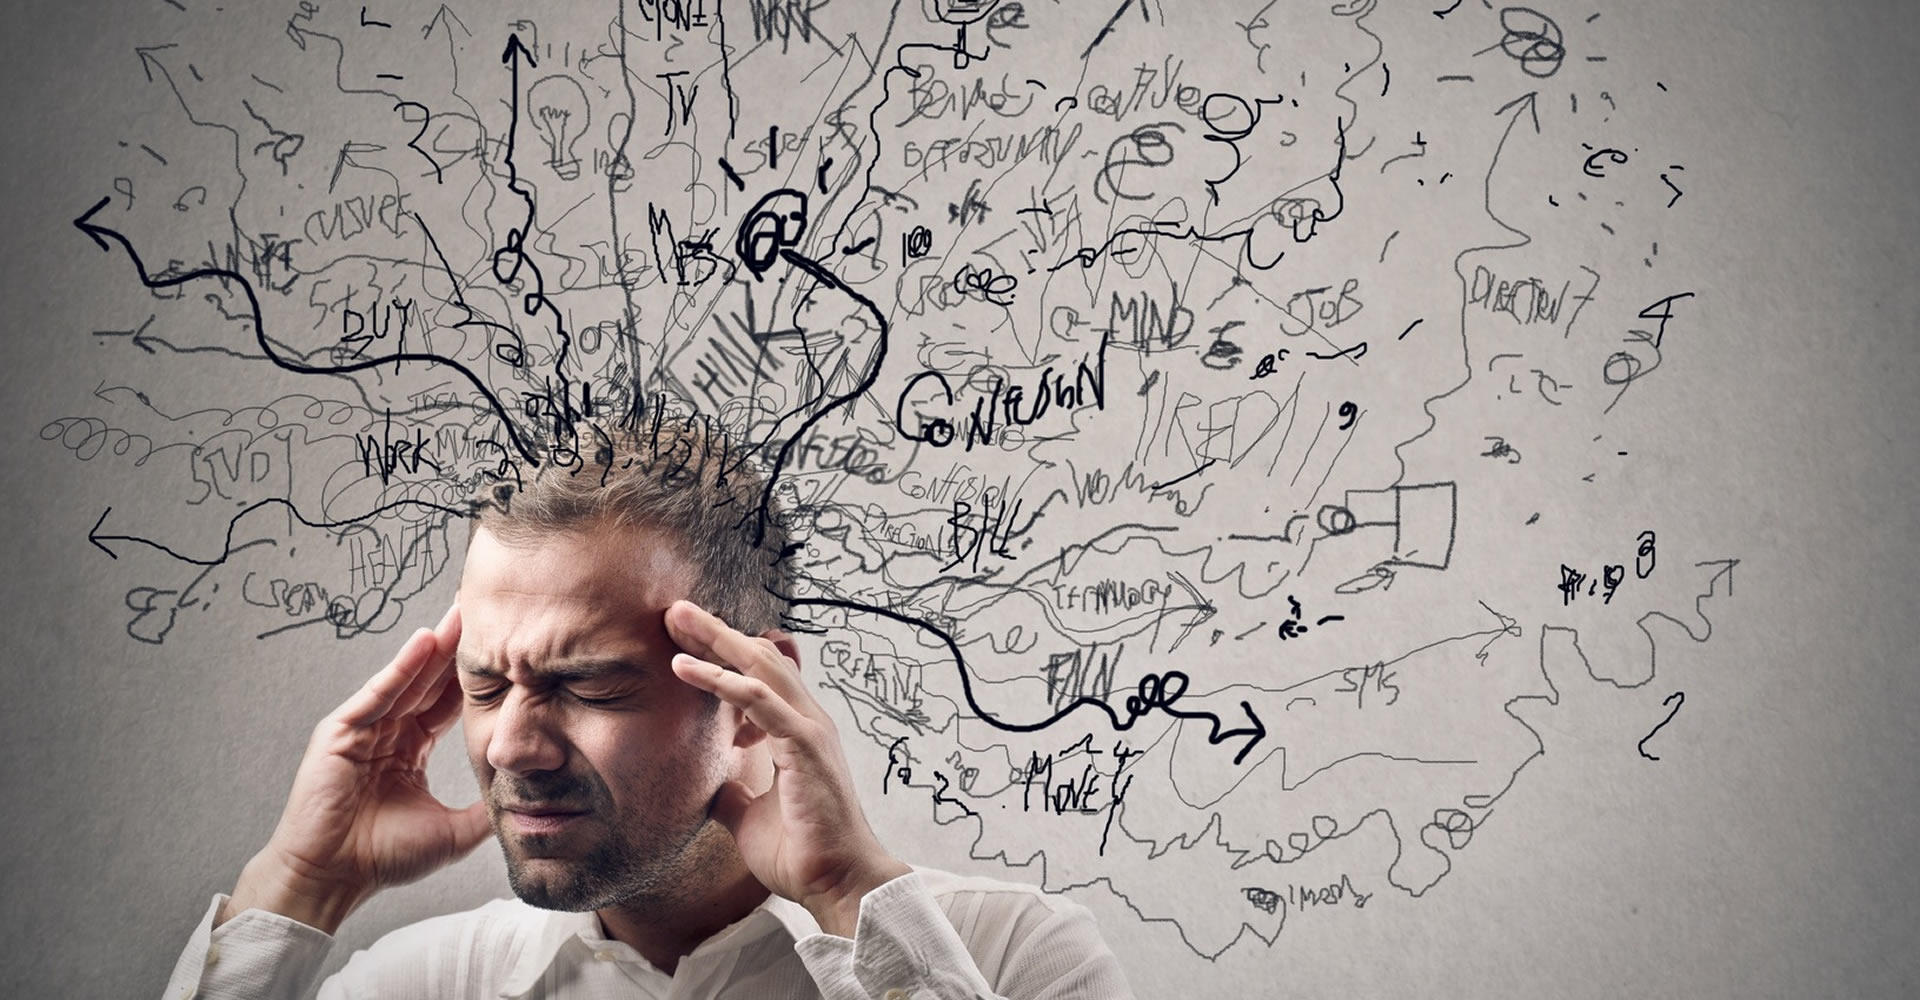
\includegraphics[width=.9\linewidth]{/Users/jay/Dropbox/github/org-html-webslides/assets/img/information-overload.jpg}
\end{center}

\section[Research room]{Research room\hfill{}\textsc{slide:full:invisible}}
\label{sec:org3f6b6f4}
\begin{center}
\includegraphics[width=.9\linewidth]{/Users/jay/Dropbox/storytelling-assets/images/icons/kill-your-darlings-nli.jpeg}
\end{center}

\section[1. \textbf{Kill} your \textbf{darlings}]{1. \textbf{Kill} your \textbf{darlings}\hfill{}\textsc{slide:image70}}
\label{sec:orgc527f00}
\begin{center}
\includegraphics[width=.9\linewidth]{/Users/jay/Dropbox/storytelling-assets/images/icons/kill-your-darlings.png}
\end{center}

\section[2. The reader is on a \textbf{need-to-know basis}]{2. The reader is on a \textbf{need-to-know basis}\hfill{}\textsc{slide:image60}}
\label{sec:org1987e84}
\begin{center}
\includegraphics[width=.9\linewidth]{/Users/jay/Dropbox/storytelling-assets/images/icons/need-to-know-basis-icon.png}
\end{center}

\section[3. Just enough fuel to keep the plane in the air]{3. Just enough fuel to keep the plane in the air\hfill{}\textsc{slide:image60}}
\label{sec:org7eb7539}
\begin{center}
\includegraphics[width=.9\linewidth]{/Users/jay/Dropbox/storytelling-assets/images/icons/plane-fuel-2.png}
\end{center}

\section[Avoiding information \textbf{overload}]{Avoiding information \textbf{overload}\hfill{}\textsc{slide:wrap:bgwhite:shadow:fancynumberedlist:compressed:image20}}
\label{sec:org0b18d51}
\begin{enumerate}
\item \textbf{Kill} your \textbf{darlings} \begin{center}
\includegraphics[width=.9\linewidth]{/Users/jay/Dropbox/storytelling-assets/images/icons/kill-your-darlings.png}
\end{center}
\item The reader is on a \textbf{need-to-know} basis \begin{center}
\includegraphics[width=.9\linewidth]{/Users/jay/Dropbox/storytelling-assets/images/icons/need-to-know-basis-icon.png}
\end{center}
\item \textbf{Just enough fuel} to keep the plane in the air \begin{center}
\includegraphics[width=.9\linewidth]{/Users/jay/Dropbox/storytelling-assets/images/icons/plane-fuel-2.png}
\end{center}
\end{enumerate}

\section[3 steps to \textbf{clarity} and \textbf{concision}]{3 steps to \textbf{clarity} and \textbf{concision}\hfill{}\textsc{slide:wrap:bgwhite:shadow:fancynumberedlist:compressed:image20}}
\label{sec:org68eca39}
\begin{enumerate}
\item Use \textbf{active} verbs \begin{center}
\includegraphics[width=.9\linewidth]{/Users/jay/Dropbox/storytelling-assets/images/icons/active-verb-icon.png}
\end{center}
\item Avoid \textbf{zombie} nouns \begin{center}
\includegraphics[width=.9\linewidth]{/Users/jay/Dropbox/storytelling-assets/images/icons/jargon-1.png}
\end{center}
\item Trim for \textbf{concision} \begin{center}
\includegraphics[width=.9\linewidth]{/Users/jay/Dropbox/storytelling-assets/images/icons/scissors-icon.png}
\end{center}
\end{enumerate}

\section[1. Use \textbf{active} verbs]{1. Use \textbf{active} verbs\hfill{}\textsc{slide}}
\label{sec:org59e0226}
\begin{center}
\includegraphics[width=.9\linewidth]{/Users/jay/Dropbox/storytelling-assets/images/icons/active-verb-icon.png}
\end{center}

\section[1. Use \textbf{active} verbs]{1. Use \textbf{active} verbs\hfill{}\textsc{slide}}
\label{sec:org7d00935}
Microsoft made the discovery that its feedback methodology failed to result in any appreciable performance improvement.

\section[1. Use \textbf{active} verbs]{1. Use \textbf{active} verbs\hfill{}\textsc{slide}}
\label{sec:orgcc10a34}
Microsoft discovered that its feedback method did not improve performance.

\section[2. Avoid \textbf{zombie} nouns]{2. Avoid \textbf{zombie} nouns\hfill{}\textsc{slide:image70}}
\label{sec:org1cb55ec}
\begin{center}
\includegraphics[width=.9\linewidth]{/Users/jay/Dropbox/storytelling-assets/images/icons/jargon-1.png}
\end{center}

\section[2. Avoid \textbf{zombie} nouns]{2. Avoid \textbf{zombie} nouns\hfill{}\textsc{slide}}
\label{sec:org2d87d03}
The rise of the planet's temperature is a result of greenhouse gases.

\section[2. Avoid \textbf{zombie} nouns]{2. Avoid \textbf{zombie} nouns\hfill{}\textsc{slide}}
\label{sec:org20abd1d}
Greenhouse gases are causing the planet's temperature to rise.

\section[2. Avoid \textbf{zombie} nouns]{2. Avoid \textbf{zombie} nouns\hfill{}\textsc{slide}}
\label{sec:orga9c779b}
Greenhouse gases are raising the planet's temperature.

\section[Exercise: \textbf{Clarity}]{Exercise: \textbf{Clarity}\hfill{}\textsc{slide:image70}}
\label{sec:org0d6669f}
\begin{center}
\includegraphics[width=.9\linewidth]{/Users/jay/Dropbox/storytelling-assets/images/icons/exercises-icon.png}
\end{center}

\section[3 steps to \textbf{clarity} and \textbf{concision}]{3 steps to \textbf{clarity} and \textbf{concision}\hfill{}\textsc{slide:wrap:bgwhite:shadow:fancynumberedlist:compressed:image20}}
\label{sec:org789e963}

\begin{enumerate}
\item Use \textbf{active} verbs \begin{center}
\includegraphics[width=.9\linewidth]{/Users/jay/Dropbox/storytelling-assets/images/icons/active-verb-icon.png}
\end{center}
\item Avoid \textbf{zombie} nouns \begin{center}
\includegraphics[width=.9\linewidth]{/Users/jay/Dropbox/storytelling-assets/images/icons/jargon-1.png}
\end{center}
\end{enumerate}

\section[3. Trim for \textbf{concision}]{3. Trim for \textbf{concision}\hfill{}\textsc{slide:image70}}
\label{sec:org0bc98ca}
\begin{center}
\includegraphics[width=.9\linewidth]{/Users/jay/Dropbox/storytelling-assets/images/icons/scissors-icon.png}
\end{center}

\section[3. Trim for \textbf{concision}]{3. Trim for \textbf{concision}\hfill{}\textsc{slide:image60}}
\label{sec:org5bc633b}
(As a separate step)

\section[3. Trim for \textbf{concision}]{3. Trim for \textbf{concision}\hfill{}\textsc{slide}}
\label{sec:orgfe0bb80}
Our biases operate in large part in order to protect us---which is why they are self-serving.

\section[3. Trim for \textbf{concision}]{3. Trim for \textbf{concision}\hfill{}\textsc{slide}}
\label{sec:org8ba910f}
Our biases are self-serving because they exist to protect us.

\section[3 steps to \textbf{clarity} and \textbf{concision}]{3 steps to \textbf{clarity} and \textbf{concision}\hfill{}\textsc{slide:wrap:bgwhite:shadow:fancynumberedlist:compressed:image20}}
\label{sec:org7708d95}
\begin{enumerate}
\item Use \textbf{active} verbs \begin{center}
\includegraphics[width=.9\linewidth]{/Users/jay/Dropbox/storytelling-assets/images/icons/active-verb-icon.png}
\end{center}
\item Avoid \textbf{zombie} nouns \begin{center}
\includegraphics[width=.9\linewidth]{/Users/jay/Dropbox/storytelling-assets/images/icons/jargon-1.png}
\end{center}
\item Trim for \textbf{concision} \begin{center}
\includegraphics[width=.9\linewidth]{/Users/jay/Dropbox/storytelling-assets/images/icons/scissors-icon.png}
\end{center}
\end{enumerate}

\section[Exercise: \textbf{Concision}]{Exercise: \textbf{Concision}\hfill{}\textsc{slide:image70}}
\label{sec:org3628aed}
\begin{center}
\includegraphics[width=.9\linewidth]{/Users/jay/Dropbox/storytelling-assets/images/icons/exercises-icon.png}
\end{center}


\section[Exercise: Problem, Agitation, Solution]{Exercise: Problem, Agitation, Solution\hfill{}\textsc{slide:image70}}
\label{sec:org6051bdc}
\begin{center}
\includegraphics[width=.9\linewidth]{/Users/jay/Dropbox/storytelling-assets/images/icons/exercises-icon.png}
\end{center}

\section[Review]{Review\hfill{}\textsc{slide:image70}}
\label{sec:org3fb65b9}
\begin{center}
\includegraphics[width=.9\linewidth]{/Users/jay/Dropbox/storytelling-assets/images/icons/memory-icon-3.png}
\end{center}

\section[\textbf{3 QUALITIES} of an effective response email]{\textbf{3 QUALITIES} of an effective response email\hfill{}\textsc{slide:wrap:bgwhite:shadow:fancynumberedlist:compressed:image20}}
\label{sec:org176806b}
\begin{enumerate}
\item \textbf{Relevant} \begin{center}
\includegraphics[width=.9\linewidth]{/Users/jay/Dropbox/github/org-html-webslides/assets/img/noun_502032_cc.png}
\end{center}
\item \textbf{Personal} \begin{center}
\includegraphics[width=.9\linewidth]{/Users/jay/Dropbox/github/org-html-webslides/assets/img/flamenco-couple-dance_318-56562.jpg}
\end{center}
\item \textbf{Persuasive} \begin{center}
\includegraphics[width=.9\linewidth]{/Users/jay/Dropbox/github/org-html-webslides/assets/img/smoker-004-512.png}
\end{center}
\end{enumerate}

\section[The Three R's of Relevance]{The Three R's of Relevance\hfill{}\textsc{slide:wrap:size60:bgwhite:shadow:flexblock:reasons:fancynumberedlist}}
\label{sec:orge297a8f}
\begin{enumerate}
\item \textbf{Responsive} Answers their question directly and explicitly.
\item \textbf{Relevant} To the prospect's situation and needs.
\item \textbf{Restrained} With no unnecessary information.
\end{enumerate}

\section[Theory of Mind]{Theory of Mind\hfill{}\textsc{slide}}
\label{sec:org231d041}
\begin{center}
\includegraphics[width=.9\linewidth]{/Users/jay/Dropbox/github/org-html-webslides/assets/img/videogame-state-levels-theory-of-mind.png}
\end{center}

\section[\textbf{Subject headers} that make people \textbf{open} and \textbf{read}]{\textbf{Subject headers} that make people \textbf{open} and \textbf{read}\hfill{}\textsc{slide}}
\label{sec:org709dcbf}

\section[Curiosity]{Curiosity\hfill{}\textsc{slide:invisible:full}}
\label{sec:org1bcdbae}
\begin{center}
\includegraphics[width=.9\linewidth]{/Users/jay/Dropbox/github/org-html-webslides/assets/img/videogame-brain-desire.png}
\end{center}

\section{Don't let the \textbf{rope} go \textbf{slack}}
\label{sec:orgb698336}
\begin{center}
\includegraphics[width=.9\linewidth]{/Users/jay/Dropbox/github/org-html-webslides/assets/img/man_heaving_on_rope.png}
\end{center}

\section[Curiosity]{Curiosity\hfill{}\textsc{slide:full}}
\label{sec:org1078964}
\begin{center}
\includegraphics[width=.9\linewidth]{/Users/jay/Dropbox/github/org-html-webslides/assets/img/curiosity-icon.jpg}
\end{center}

\section[The \textbf{Elements} of \textbf{Storytelling}]{The \textbf{Elements} of \textbf{Storytelling}\hfill{}\textsc{slide:wrap:bgwhite:shadow:fancynumberedlist:compressed:image10}}
\label{sec:org0df550f}

\section[The \textbf{Elements} of \textbf{Storytelling}]{The \textbf{Elements} of \textbf{Storytelling}\hfill{}\textsc{slide:wrap:bgwhite:shadow:fancynumberedlist:compressed:image10}}
\label{sec:org90a9f05}
\begin{enumerate}
\item Goal \begin{center}
\includegraphics[width=.9\linewidth]{/Users/jay/Dropbox/github/org-html-webslides/assets/storytelling-icons/goal.png}
\end{center}
\item Obstacle \begin{center}
\includegraphics[width=.9\linewidth]{/Users/jay/Dropbox/github/org-html-webslides/assets/storytelling-icons/obstacle.png}
\end{center}
\item Stakes \begin{center}
\includegraphics[width=.9\linewidth]{/Users/jay/Dropbox/github/org-html-webslides/assets/storytelling-icons/stakes.png}
\end{center}
\item Strategies \begin{center}
\includegraphics[width=.9\linewidth]{/Users/jay/Dropbox/github/org-html-webslides/assets/storytelling-icons/strategies.png}
\end{center}
\item Outcome \begin{center}
\includegraphics[width=.9\linewidth]{/Users/jay/Dropbox/github/org-html-webslides/assets/storytelling-icons/outcome.png}
\end{center}
\end{enumerate}

\section{\textbf{2 Structures} for a Sales Email}
\label{sec:org384ee6f}

\section[Problem / Agitation / Solution]{Problem / Agitation / Solution\hfill{}\textsc{slide:wrap:bgwhite:shadow:fancynumberedlist:compressed:image30}}
\label{sec:org8fba461}
\begin{enumerate}
\item Problem \begin{center}
\includegraphics[width=.9\linewidth]{/Users/jay/Dropbox/github/org-html-webslides/assets/img/3d-problem.png}
\end{center}
\item Agitation \begin{center}
\includegraphics[width=.9\linewidth]{/Users/jay/Dropbox/github/org-html-webslides/assets/img/3d-agitation-your-life-sucks.png}
\end{center}
\item Solution \begin{center}
\includegraphics[width=.9\linewidth]{/Users/jay/Dropbox/storytelling-assets/images/3d-solution.jpg}
\end{center}
\end{enumerate}


\section[Opportunity / Benefits / Solution]{Opportunity / Benefits / Solution\hfill{}\textsc{slide:wrap:bgwhite:shadow:fancynumberedlist:compressed:image20}}
\label{sec:org6e09de5}
\begin{enumerate}
\item Opportunity \begin{center}
\includegraphics[width=.9\linewidth]{/Users/jay/Dropbox/storytelling-assets/images/icons/noun_diamond-object-of-desire.png}
\end{center}
\item Benefits \begin{center}
\includegraphics[width=.9\linewidth]{/Users/jay/Dropbox/storytelling-assets/images/icons/benefits-icon.png}
\end{center}
\item Solution \begin{center}
\includegraphics[width=.9\linewidth]{/Users/jay/Dropbox/storytelling-assets/images/icons/solution-icon.png}
\end{center}
\end{enumerate}

\section[3 steps to \textbf{clarity} and \textbf{precision}]{3 steps to \textbf{clarity} and \textbf{precision}\hfill{}\textsc{slide:wrap:bgwhite:shadow:fancynumberedlist:compressed:image20}}
\label{sec:org747ccaa}
\begin{enumerate}
\item Use \textbf{active} verbs \begin{center}
\includegraphics[width=.9\linewidth]{/Users/jay/Dropbox/storytelling-assets/images/icons/active-verb-icon.png}
\end{center}
\item Avoid \textbf{zombie} nouns \begin{center}
\includegraphics[width=.9\linewidth]{/Users/jay/Dropbox/storytelling-assets/images/icons/jargon-1.png}
\end{center}
\item Trim for \textbf{concision} \begin{center}
\includegraphics[width=.9\linewidth]{/Users/jay/Dropbox/storytelling-assets/images/icons/scissors-icon.png}
\end{center}
\end{enumerate}


\section[Effective Emails]{Effective Emails\hfill{}\textsc{slide:aligncenter}}
\label{sec:org9146cf3}

\textbf{Jay Dixit} \\
\href{http://www.storytelling.nyc}{www.storytelling.nyc} \\
\href{mailto:jay@storytelling.nyc}{jay@storytelling.nyc} \\

\begin{center}
\includegraphics[width=.9\linewidth]{/Users/jay/Dropbox/github/org-html-webslides/assets/img/storytelling-nyc-logo-new-face.png}
\end{center}

\section[The End]{The End\hfill{}\textsc{slide}}
\label{sec:orga3bf4b2}
\end{document}
